\section{Use Case 2: Roadwarrior}
Im diesem Use-Case soll erarbeitet werden, inwefern sich Mitarbeiter via VPN - im Folgenden Roadwarrior genannt - mit den zuvor ausgerollten Cloud-Infrastrukturen verbinden können. Ralf Spenneberg definiert diesen Begriff wie folgt:\\
\glqq Der Begriff Roadwarrior bezeichnet Personen, die mit unbestimmter IP-Adresse auf ein VPN-Gateway zugreifen wollen. Typischerweise handelt es sich hierbei zum Beispiel um Außendienstmitarbeiter, die von unterwgs Zugriff auf die Datenbanken ihres Mutterunternehmens benötigen. Aber auch alle anderen Konstellation, bei denen Rechner mit dynamischen IP-Adressen eine VPN-Verbindung mit einem VPN-Gateway aufbauen möchten, sind denkbar. Hierbei ist die Anzahl der Roadwarrior nicht beschränkt. Theoretisch und auch praktisch sind mehrere Hundert gleichzeitiger Tunnel möglich.\grqq{} \cite[S. 199]{Spenneberg2010}\\
Gerade die Corona-Krise hat das Ausweichen auf das Home-Office für einige Branchen unverzichtbar gemacht. Einige prophezeien bereits eine neue Arbeitswelt \textit{New Work}, die \glqq flexible Arbeitsgestaltung, zum Beispiel durch Vertrauensarbeitszeit und -orte sowie Verzicht auf standardisierte Kernarbeitszeiten\grqq{} mit sich bringt \cite{Umbs2020}.
Klassischerweise verbindet sich der Roadwarrior mit dem Hauptstandort, um von dort aus weitere interne Ressourcen zu erreichen - in diesem Falle die Private Cloud. Dieses klassische Design bringt insbesondere unter der Annahme, dass sich Dienste in die Cloud verlagern lassen (Use-Case 3?), diverse Probleme mit sich:
%Auf Corona-Zeiten eingehen...

\begin{itemize}
%https://tu-freiberg.de/urz/bandbreite-des-vpn-zugangs-verzehnfacht
\item Der Hautpstandort muss Bandbreite für alle n Roadwarrior zur Verfügung stellen. V.a. in zu Beginn der Corona-Krise durften viele Unternehmen erfahren, dass sie hier schlecht aufgestellt sind.
\item Der Hauptstandort ist u.U. weit entfernt. Der Mitarbeiter nimmt auf Grund von hohen Latenzen und eventuellen Paketverlusten eine schlechte Applikations-Performance wahr. Oftmals wird über Smartphone-Hotspot, Hotel-WLAN, o.ä. gearbeitet. 
%Fulltunnel als Argument?
\item Latenzen erhöhen sich zusätzlich, falls bestimmte Applikations-Server gar nicht am Hauptstandort vorhanden sind, z.B. weil sie in die Public Cloud verlagert wurden.
\end{itemize}

Optimalerweise wird das Design also diese genannten Punkte in Angriff nehmen:\\

\begin{itemize}
\item Ein Load Balancing der Bandbreiten wird ermöglicht, indem n Roadwarrior über m Clouds verteilt werden.
\item Der Roadwarrior verbindet sich im günstigsten Fall mit dem Standort, der die geringste Entfernung zu ihm aufweist.
\item Viel genutzte Applikationen sind am jeweiligen Cloud-Standort, mit dem sich der Roadwarrior verbunden hat, verfügbar, um eine gute Usability für den Anwender zu gewährleisten.
\item Weiterhin sollen genannte Maßnahmen für den Anwender möglichst transparent und ohne manuelle Interaktion erfolgen. Er soll keine Wahl haben, mit welchem Cloud-Standort er sich zu verbinden hat: die Annahme ist, dass dieser über geeignete Automatisierungsmechanismen mit dem \textit{besten} Standort verbunden wird.
\end{itemize}

Das Szenario baut auf Use-Case 1 auf. So wird weiterhin von dem Backbone-Grundaufbau ausgegangen. Es soll gezeigt werden, wie ein Roadwarrior-Setup aufgebaut werden kann, bei dem sich der jeweilige Mitarbeiter mit dem nächstgelegen \textit{Hop} verbindet, um die beste Performance erreichen zu können. Weiterhin soll an jedem Cloud-Standort ein (interner) Server stehen, der den gleichen Dienst anbietet. Das Ziel ist es, dass ausschließlich der Server genutzt wird, der an dem Standort zur Verfügung steht. Ansonsten würden sich der Latenzgewinn durch die nahe VPN-Gegenstelle durch die \textit{interne} Latenz wieder aufheben.

Die Infrastruktur-Komponenten aus Use-Case 1 werden als vorhanden und funktionierend angenommen und im folgenden Bild nicht mehr dargestellt. Die Roadwarrior-Clients verbinden sich immer mit dem nächstgelegenen VPN-Konzentrator.

\begin{figure}[h]
  \centering
  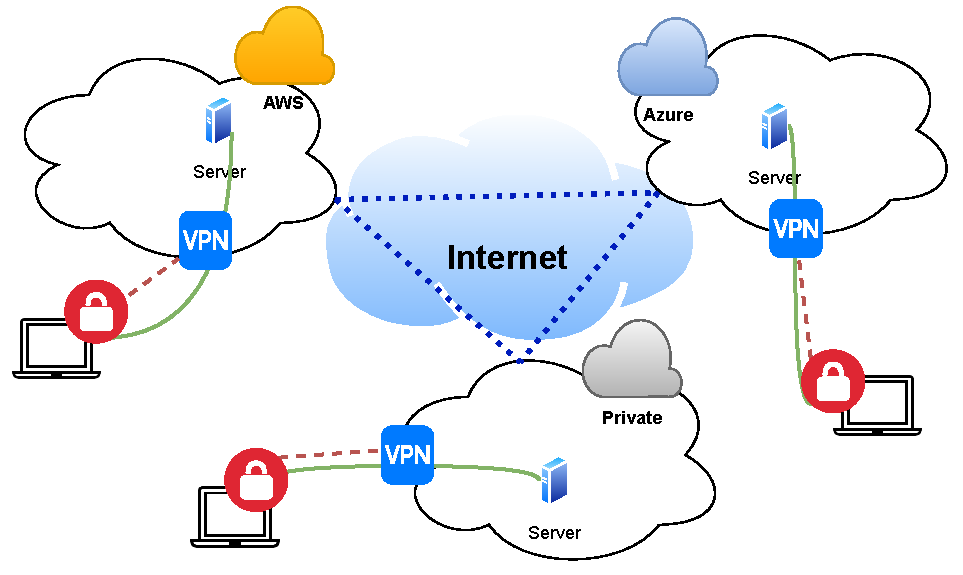
\includegraphics{Figures/Use-Case_2_Vereinfacht_1.pdf}
  \caption{Use-Case 2: Roadwarrior}
  \label{grafik:Use-Case-2_Vereinfacht}
\end{figure}

\subsection{Vorauswahl geeigneter technischer Komponenten}
Zur Terminierung der Roadwarrior-Clients muss pro Cloud-Standort ein VPN-Konzentrator zur Verfügung stehen. Mit \textit{Client VPN Endpoint} (AWS) bzw. \textit{Point-to-site} Azure bieten bereits Lösungen, um Roadwarrior-Clients zu terminieren. Nach längerer Evaluation dieser Building Blocks erwiesen sich diese Lösungen für das Ziel der Arbeit als nicht tauglich:
\begin{itemize}
\item Bei AWS werden Client-VPN-Verbindungen eingehend geNATted (\texit{NAT Masquerading}). Damit sind alle Clients intern mit der gleichen Absender-IP zu sehen. Dies verletzt den Anspruch der Arbeit, eine Ende-zu-Ende-Konnektivität zu ermöglichen.
\item Obwohl Azure als auch AWS OpenVPN für Roadwarrior-VPNs benutzen, sind die Client-VPN-Konfigurationen nicht \glqq deckungsgleich\grqq{} zu bekommen. Um den sich mit dem nächstgelegenen VPN-Konzentrator zu verbinden, wäre eine manuelle Interaktion des Benutzers notwendig, was mit den Evaluationskriterien nicht vereinbar ist. Weiterhin kann der Benutzer nicht immer wissen, wo der nächstgelegene Standort ist. Man kann nicht von jedem Mitarbeiter tiefe Topologiekenntnisse des Netzwerks abverlangen.
\end{itemize}

AWS benutzt bspw. eine \textit{remote-random-hostname}-Direktive, welche dafür sorgt, dass bei Verbindungsversuch eine Zufallszeichenkette an den Domainnamen angehanden wird, um DNS Caching zu verhindern.
\begin{lstlisting}[label=ovpn_configs_aws_azure,caption=Auszüge aus den OpenVPN-Client-Konfigurationen für AWS und Azure]
$ grep remote *-client-vpn.ovpn
aws-client-vpn.ovpn:remote cvpn-endpoint-08345654356c59c40.prod.clientvpn.eu-central-1.amazonaws.com 443
aws-client-vpn.ovpn:remote-random-hostname
aws-client-vpn.ovpn:remote-cert-tls server
azure-client-vpn.ovpn:remote azuregateway-61820068-8212-4781-af1a-788136407c66-252bb491f2e5.vpn.azure.com 443
azure-client-vpn.ovpn:remote-cert-tls server
\end{lstlisting}

Weiterhin sind die unterschiedlichen Authentifizierungsmechanismen nur schwierig miteinander zu kombinieren. Auch hier wäre eine Benutzerinteraktion notwendig.

Daher wurde für weitere Überlegungen von den offiziellen Building-Blocks abgesehen und entschieden, pro Standort einen eigenen OpenVPN-Server hochzufahren:
OpenVPN ist freie Software und man muss sich daher nicht mit Lizenzierungen beschäftigen analog zu VyOS. Weiterhin sind die Konfigurationen sehr gut automatisierbar: Der OpenVPN-Server benötigt ausschließlich eine textuale Konfigurationsdatei, welche sich gut aus einem Terraform-Template erzeugen ließe.
%RADIUS
Ein Problem ergibt sich aus der Authentifizierung und Autorisierung der Roadwarrior-Clients. Wenn Protokolle wie RADIUS als Authentifizierungsmechanismus mit Benutzerkennung und Passwort, muss man entweder\\
a) einen zentralen RADIUS-Server pro Standort verwalten oder \\
b) einen zentralen RADIUS-Server für alle Standorte zur Verfügung stellen.\\

a) bringt ein Skalierungsproblem mit sich. So müssen bspw. Benutzerkennungen und Passwörter lokal auf allen Systemen gepflegt werden, was die Komplexität des Use-Cases deutlich erhöhen würde und auch in Realität schwierig zu warten wäre. Mit b) hätte man einen Single-Point-of-Failure, scheidet also auch aus. Hätte der \textit{zentrale} Authentifizierungsserver ein technisches Problem, wären alle VPN-Konzentratoren betroffen und Roadwarrior könnten sich nicht mehr einwählen.

%LDAP allgemein???
LDAP als verteilte Datenbank wäre eine Lösung für genannte Probleme: man müsste pro Standort einen LDAP-Server deployen und durchgehend mit allen weiteren LDAP-Servern synchronisieren. Als Authentifizierungsmechanismus könnte man dann RADIUS oder gleich LDAP benutzen. Windows Domain Controller wäre ein Beispiel für solch ein Szenario. In der Bachelorarbeit wird auch davon abgesehen, da die Komplexität deutlich erhöht und es für den Proof-of-Concept an sich keine gewinnbringenden Erkenntnisse liefern würde.

%Kurzeinstieg PKI?
Der Lösungsansatz wäre, auf eine Zertifikat-basierte Authentifizierung zu setzen. Eine Publik-Key-Infrastruktur benötigt zur Authentifizierung keine Verbindungen zu anderen (Authentifizierungs-)Services. Es reicht, auf dem VPN-Server vertrauenswürdige Root-Zertifikate zu hinterlegen. Diese \textit{vertrauenswürdigen Stellen} signieren mit dem privaten Schlüssel dann die Zertifikate der Roadwarrior-Clients, wodurch das Vertrauensverhältnis zwischen VPN-Server und -Client hergestellt ist.\\
Auf Prüfung der Gültigkeit von Zertifikaten mittels Certificate Revocation Lists (CRLs) bzw. Online Certificate Status Protocol (OCSP) wird in dieser Bachelor-Arbeit verzichtet. Sie ist aber prinzipiell möglich mit der serverseitigen OpenVPN-Direktive \textit{crl-verify} (CRL-Prüfung) bzw. \textit{tls-verify} (OCSP-Prüfung).\cite[S.116, S. 325-327]{Keijser2011}
\ifFalse
Ein Grenzfall wäre durch die Funktion wie Domain Controller (DC) bei Windows Active Directory gegeben. Dieser kann dezentral an allen Standorten deployed werden und bringt eine RADIUS-Server-Rolle (Network Policy Server) mit. Sobald Domänenbenutzer hinzugefügt / gelöscht / geändert werden, würden alle DCs an den verschiedenen Standorten automatisch über das Active Directory über diese Änderung informiert. Network Policy Server als RADIUS-Server könnte lokal Benutzerkennung und Passwort prüfen. Windows Active Directory ist ein Spezialfall von Lightweight Directory Access Protocol. Weitere LDAP-Lösungen bringen solche Synchronisationsmechanismen mit, haben allerdings keine RADIUS-Funktionalität gibt es weitere dezentrale...\\
\fi


%Authentisierung
%GeoIP vs. Anycast, bspw. Google DNS 8.8.8.8 -> warum ist das hier nicht praktibel (Kunden haben keine eigenen Netze und peeren nicht weltweit)
%
%AWS == Frankfurt, Azure == Dublin, Kiel
%CRL / OCSP
\subsection{Evaluationskriterien}
\begin{itemize}
\item Roadwarrior-Clients werden simuliert, indem an den entsprechenden Standort (Kiel, Dublin bzw. Frankfurt) eine weitere virtuelle Maschine installiert wird, die VPN-Verbindungen zu den jeweiligen Konzentratoren aufbaut.
\item Ein Roadwarrior-Client verbindet sich immer mit dem nächstgelegen Standort. Die DNS-Antworten werden per \texit{dig}- und \textit{whois}-Kommando verifiziert.
\item Der Client hat keine Wahl, mit welchem Standort dieser verbunden wird.
\item Ist ein Cloud-Standort nicht verfügbar (z.B. weil defekt oder nicht deployed), muss der Client auf den \textit{default} Standort (Kiel) zurückfallen.
\item Sobald ein Client mit einem VPN verbunden ist, muss er die entsprechende interne Server-Ressource ansprechen, die am jeweiligen Standort zur Verfügung steht.
\end{itemize}
